\documentclass[12pt]{article}
\usepackage[margin=2.5cm]{geometry}
\usepackage{enumerate}
\usepackage{amsfonts}
\usepackage{amsmath}
\usepackage{fancyhdr}
\usepackage{amsmath}
\usepackage{amssymb}
\usepackage{amsthm}
\usepackage{mdframed}
\usepackage{graphicx}
\usepackage{subcaption}
\usepackage{listings}
\usepackage{xcolor}
\usepackage[utf]{kotex}

\definecolor{codegreen}{rgb}{0,0.6,0}
\definecolor{codegray}{rgb}{0.5,0.5,0.5}
\definecolor{codepurple}{rgb}{0.58,0,0.82}
\definecolor{backcolour}{rgb}{0.95,0.95,0.92}

\lstdefinestyle{mystyle}{
    backgroundcolor=\color{backcolour},
    commentstyle=\color{codegreen},
    keywordstyle=\color{magenta},
    numberstyle=\tiny\color{codegray},
    stringstyle=\color{codepurple},
    basicstyle=\ttfamily\footnotesize,
    breakatwhitespace=false,
    breaklines=true,
    captionpos=b,
    keepspaces=true,
    numbers=left,
    numbersep=5pt,
    showspaces=false,
    showstringspaces=false,
    showtabs=false,
    tabsize=1
}

\lstset{style=mystyle}

\begin{document}
\title{CSC148 Worksheet 3 Solution}
\author{Hyungmo Gu}
\maketitle

\section*{Question 1}
\begin{enumerate}[i.]
    \item

    The memory diagram for this code is the following

    \begin{center}
    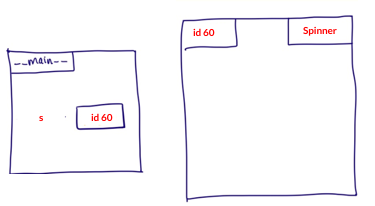
\includegraphics[width=0.7\linewidth]{images/worksheet_3_q1a_solution.png}
    \end{center}

    \begin{mdframed}
        \underline{\textbf{Correct Solution:}}

        \bigskip

        \begin{center}
        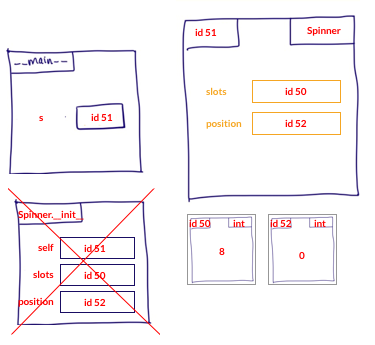
\includegraphics[width=0.7\linewidth]{images/worksheet_3_q1a_correction.png}
        \end{center}
    \end{mdframed}

    \bigskip

    \textbf{Notes:}

    \begin{itemize}
    \item Noticed that professor assigns id in order of execution.
    \item Is there a source or tutorial where this concept can be practiced?
    I feel super shaky about the concepts of memory model :(.
    \item Learned that attribute types in an object can be declared as following

    \begin{lstlisting}[language=Python]
    from datetime import date


    class Tweet:
        """A tweet, like in Twitter.

        === Attributes ===
        content: the contents of the tweet.
        userid: the id of the user who wrote the tweet.
        created_at: the date the tweet was written.
        likes: the number of likes this tweet has received.
        """
        # Attribute types
        userid: str
        created_at: date
        content: str
        likes: int
    \end{lstlisting}

    \item Learned that attribute types doesn't create variables on initialization.
    \end{itemize}

    \item The initializer of Spinner class creates variables 'slots' and 'position' at
    global level

    \bigskip

    \begin{mdframed}
        \underline{\textbf{Attempt 2:}}

        \bigskip

        The initializer of Spinner class creates variables 'slots' and 'position' at
    \color{red}local level within the method\color{black}.
    \end{mdframed}

    \item AttributeError is raised when doctest is run.
\end{enumerate}

\section*{Question 2}

\section*{Question 3}

\end{document}